%Wie eingangs er-wähnt, definieren die Anforderungen, was das System zu
%leisten hat, während die Funktionalitä-ten definieren, wie das System diese gewährleistet.
\chapter{Interface-Design}
\label{chapter-design}
Neben den inhaltlichen Funktionalitäten ist im menschzentrierten Gestaltungsprozess vor allem die
Gestaltung des Interface-Designs und -Komponenten von zentraler Bedeutung (DIN EN ISO 9241-210,
2011). Das Design sollte so entwickelt werden, dass es möglichst optimal die aus
\ref{chapter-konzept} entwickelten Funktionalitäten berücksichtigt. Folglich sollten die in 
\ref*{section:benutzer} erarbeiteten Nutzenden die Gestaltungslösungen verstehen und bedienen können. Hierbei
spielen insbesondere Komponenten wie Ein- und Ausgabemöglichkeiten, Systemfeedback sowie Farben,
Formen und Anordnungen eine Rolle. Daher wurden die acht goldenen Regeln nach
\citeA{shneiderman_designing_1997} und die Zehn Usability Heuristiken nach \citeA{nielsen_enhancing_1994}
bei der Entwicklung stets mit eingearbeitet und zur Begründung herangezogen.

Die Medieninformatik beinhaltet viele Methoden und Vorgehensweisen zur menschzentrierten Gestaltung
\todo{(Herczeg, 2006)}. Im Rahmen der Arbeit wurde vor allem Prototyping in verschiedenen Formen
eingesetzt \todo{(Herczeg, 2009a)}.

Im Folgenden wird auf den Gestaltungsprozess genauer eingegangen und gezeigt, wie die Komponenten für
das entwickelte System konzipiert und ausgestaltet wurden.

\section{Erste Iteration: Skizzen}
Die erste Iteration des Interface-Designs umfasst Skizzen. Diese sollen die grobe Anordnung der
Komponenten veranschaulichen. Daher wurde sich entstspechend auf diese fokussiert und das Farbschema zunächst
vernachlässigt. Die Skizzen wurden in Mockup\footnote{\url{https://getmockup.app/}} umgesetzt. 

In der Gestaltung wurde nach der \enquote{Mobile First}-Strategie gearbeitet (\anfref{R40}). Dieser
besagt die Nutzung der Bildschirmfläche zur schrittweisen Verbesserung von Darstellung und Inhalt
\cite{kim_chapter_2013}.


Bei der Anordnung der Komponenten wurde sich an aus den Iterviews orientieren Apps, wie
Airbnb\footnote{\url{https://www.airbnb.de/}} und Otto\footnote{\url{https://www.otto.de/}}
orientieren. Des Weiteren wurden Tailwind UI\footnote{\url{https://tailwindui.com/components}} und
Headless UI\footnote{\url{https://headlessui.com/}} als
Inspirationsquelle genutzt, um die Realisierung des Systems zu erleichtern. 

\ref{fig:m0} zeigt die Anmeldung (Ft-VA-1). Mitte ist das Dashboard der Anwendung
zu sehen (Ft-VA-1, Ft-VA-6). Rechts zeigt die Navigation (Ft-VA-1).

\begin{figure}[h]
    \centering
    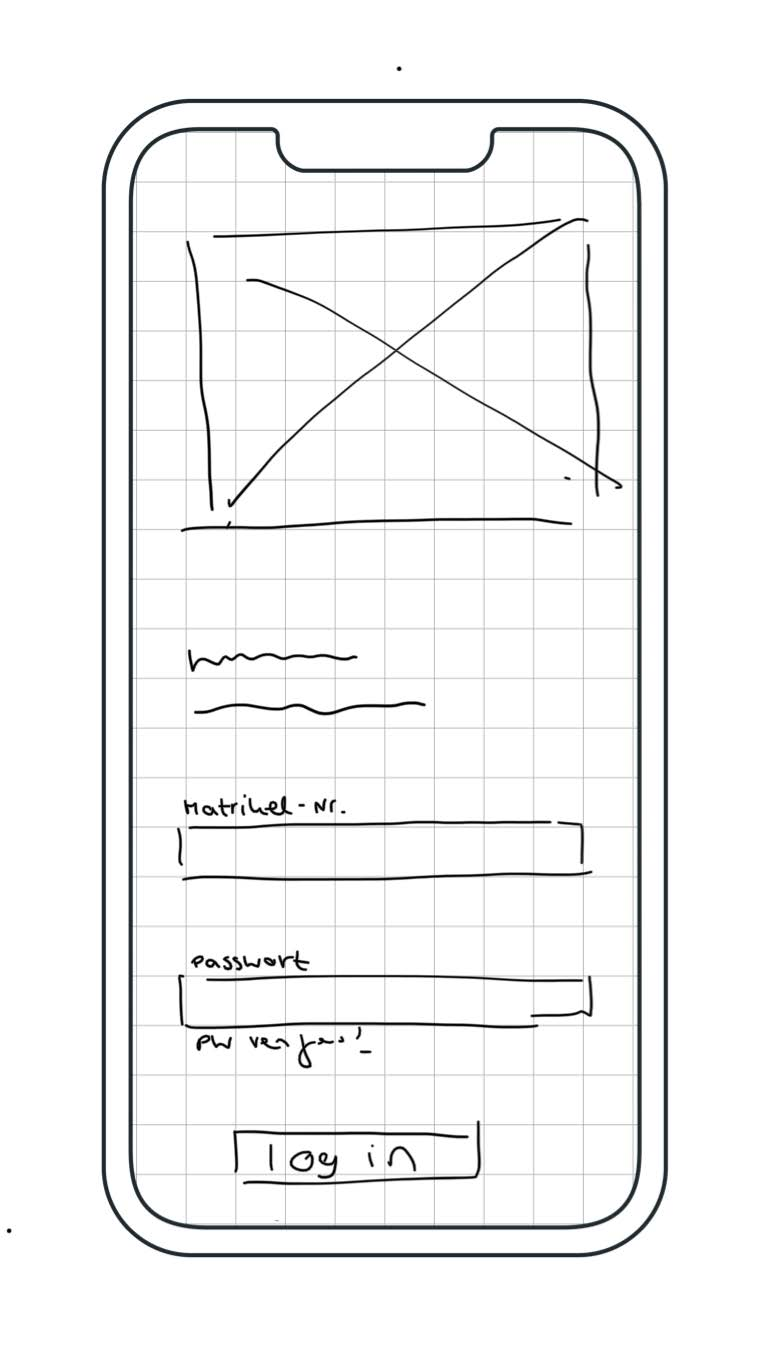
\includegraphics[scale=0.37]{Bilder/Mockups/Login.jpg}
    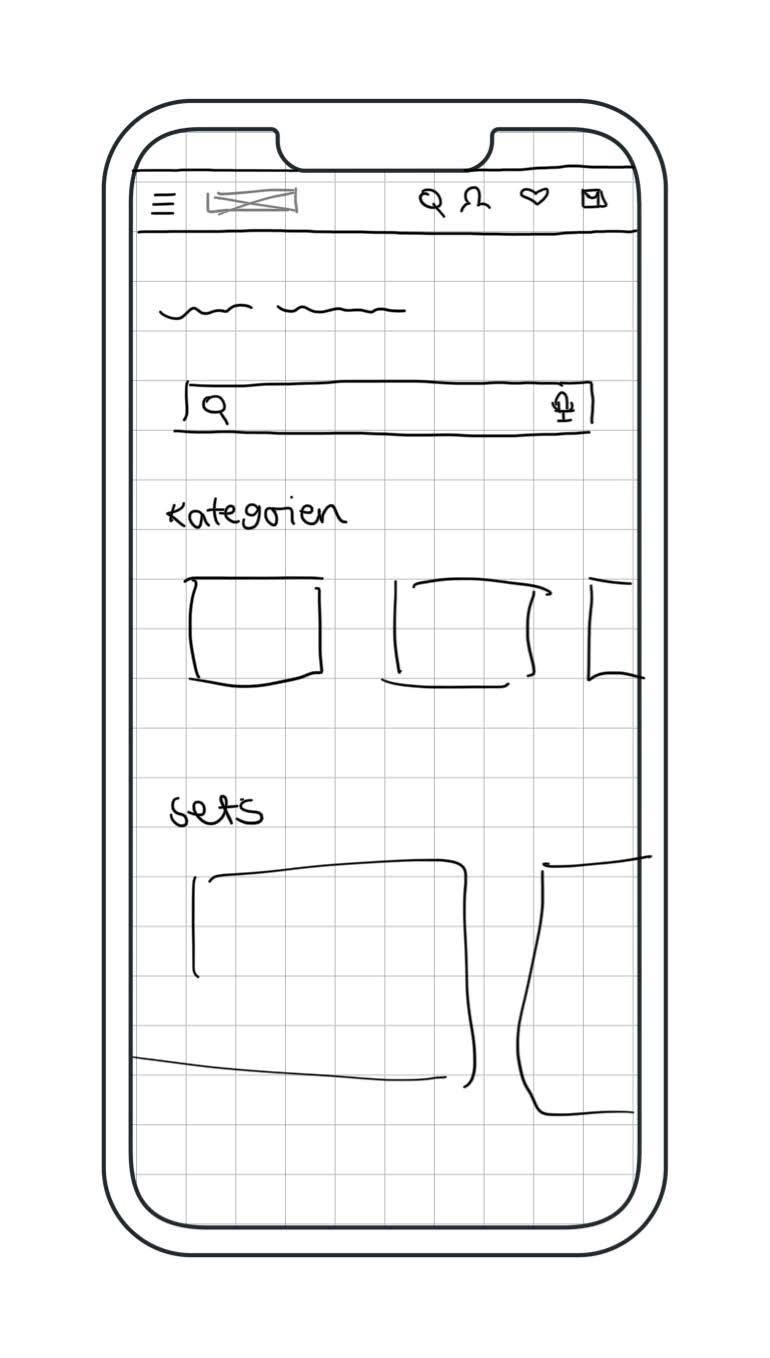
\includegraphics[scale=0.37]{Bilder/Mockups/Hom.jpg}
    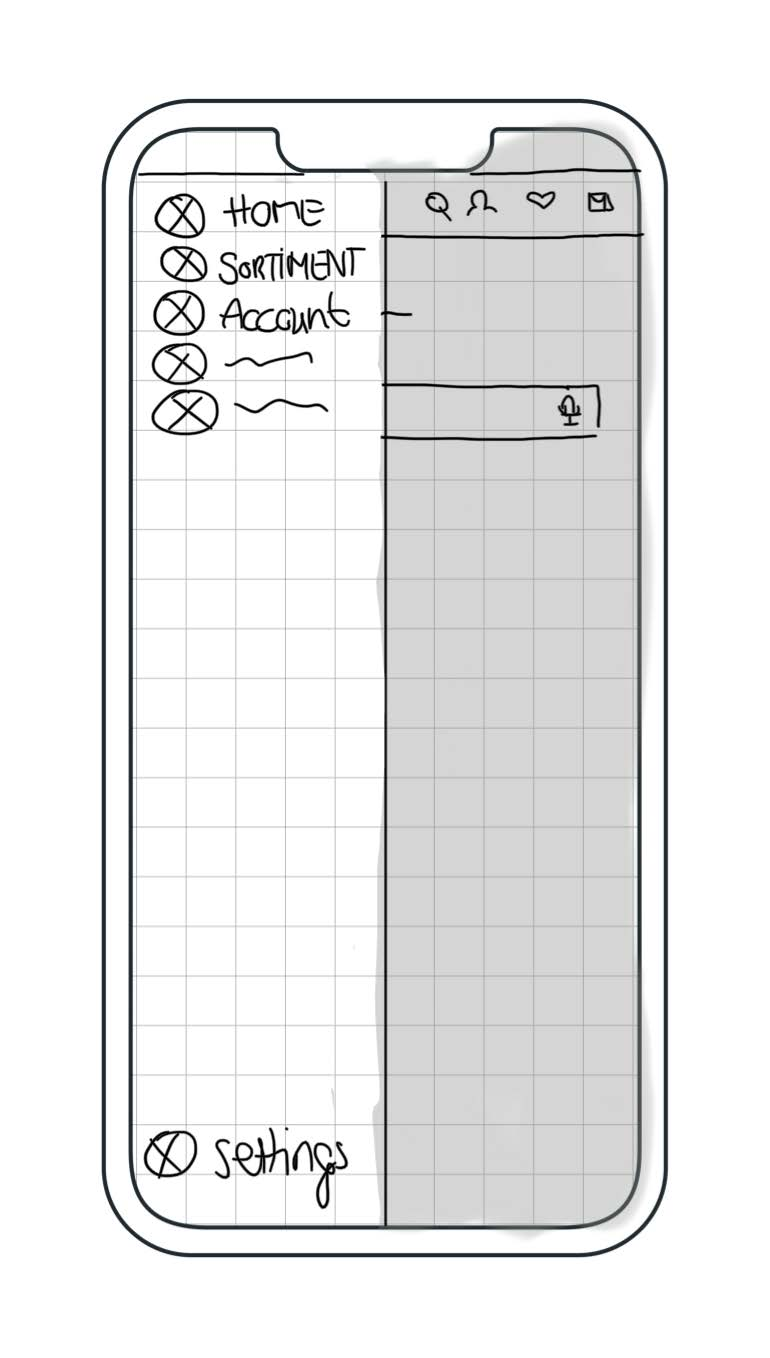
\includegraphics[scale=0.37]{Bilder/Mockups/Navbar.jpg}
    \label{fig:m0}
\caption[Mockup: Anmeldung, Dashboard, Navigation]{Anmeldung (l), Dashboard (m), Navigation (r)}
\end{figure}


\ref{fig:m0} zeigt die Kategorien (Ft-VA-2). Mitte zeigt die Assets im Überblick, mit Status
(Ft-VA-2, Ft-VA-3, Ft-VA-7). Rechts zeigt die Assetdetails der Anwendung zu sehen (Ft-VA-4,
Ft-VA-8). 


\begin{figure}[h]
    \centering
    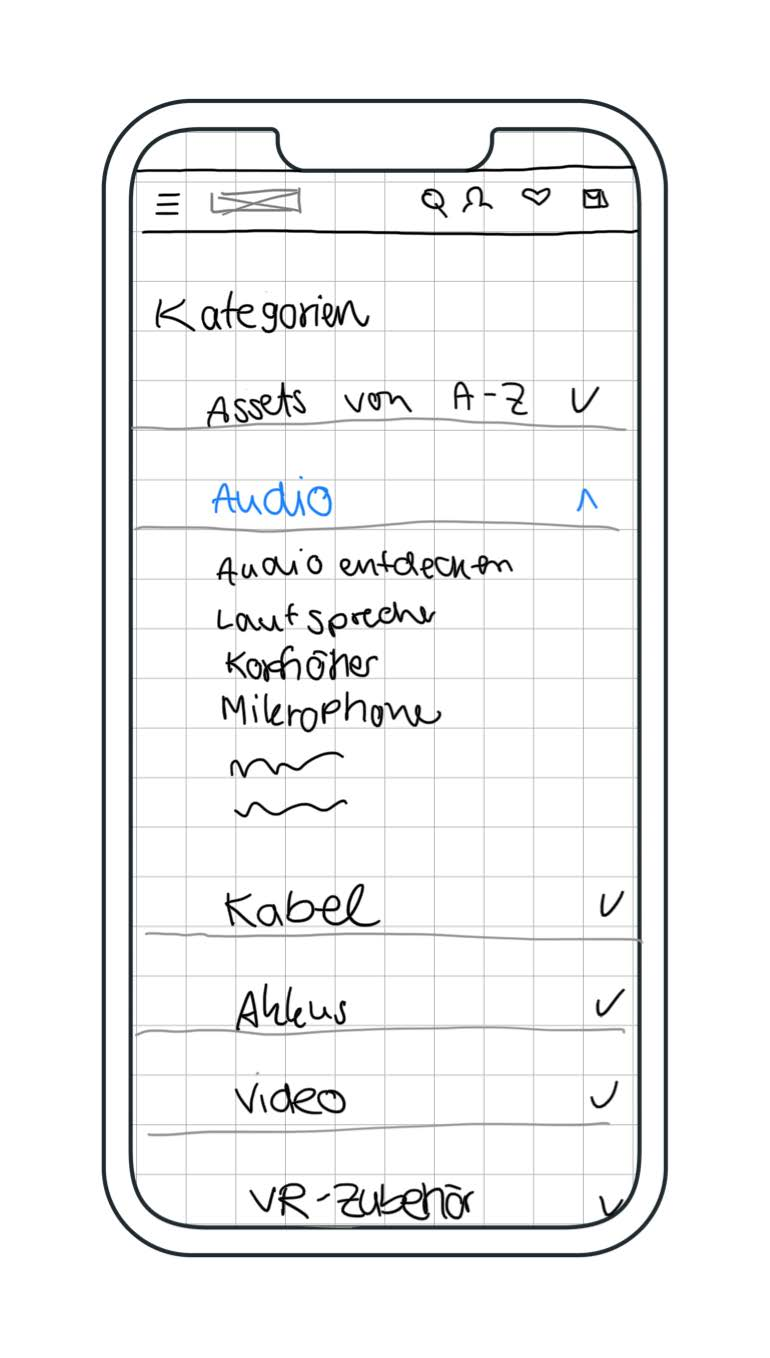
\includegraphics[scale=0.37]{Bilder/Mockups/Kategorien.jpg}
    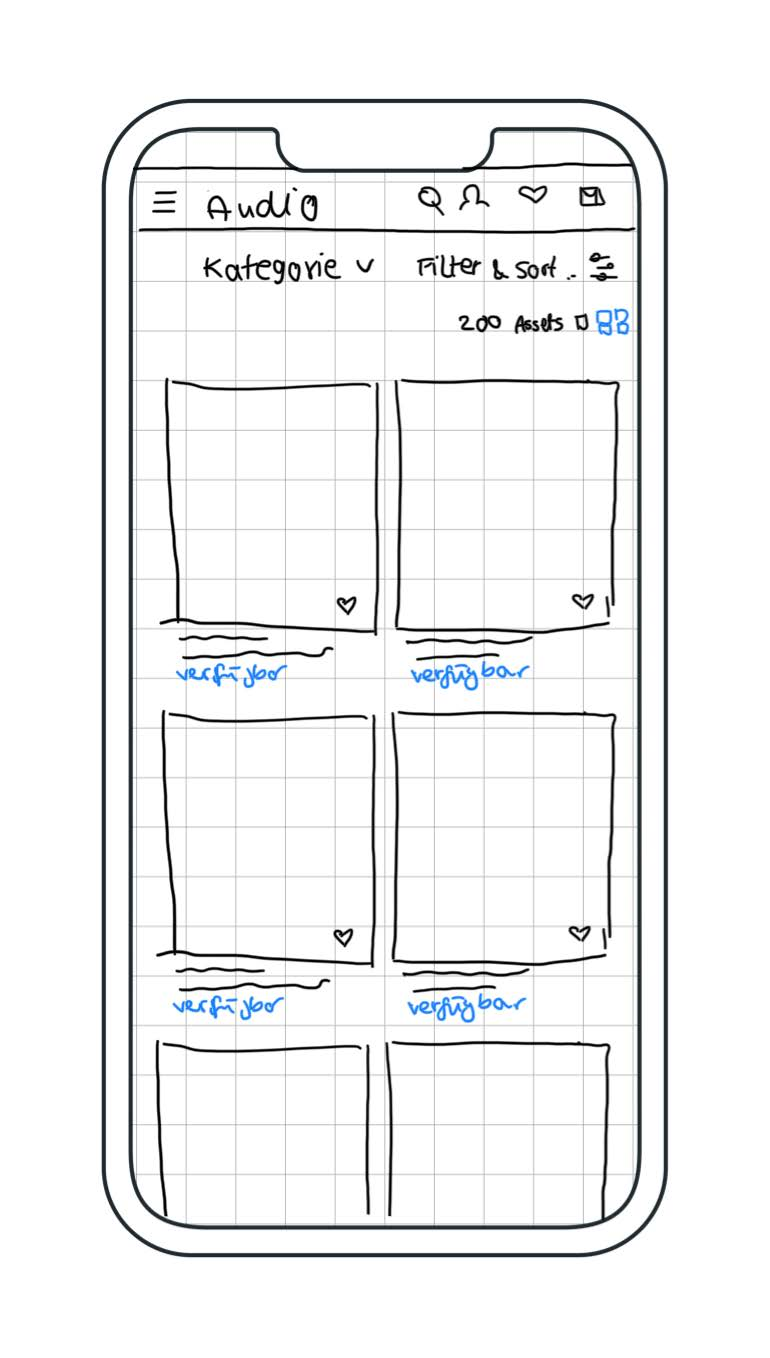
\includegraphics[scale=0.37]{Bilder/Mockups/Kacheln.jpg}
    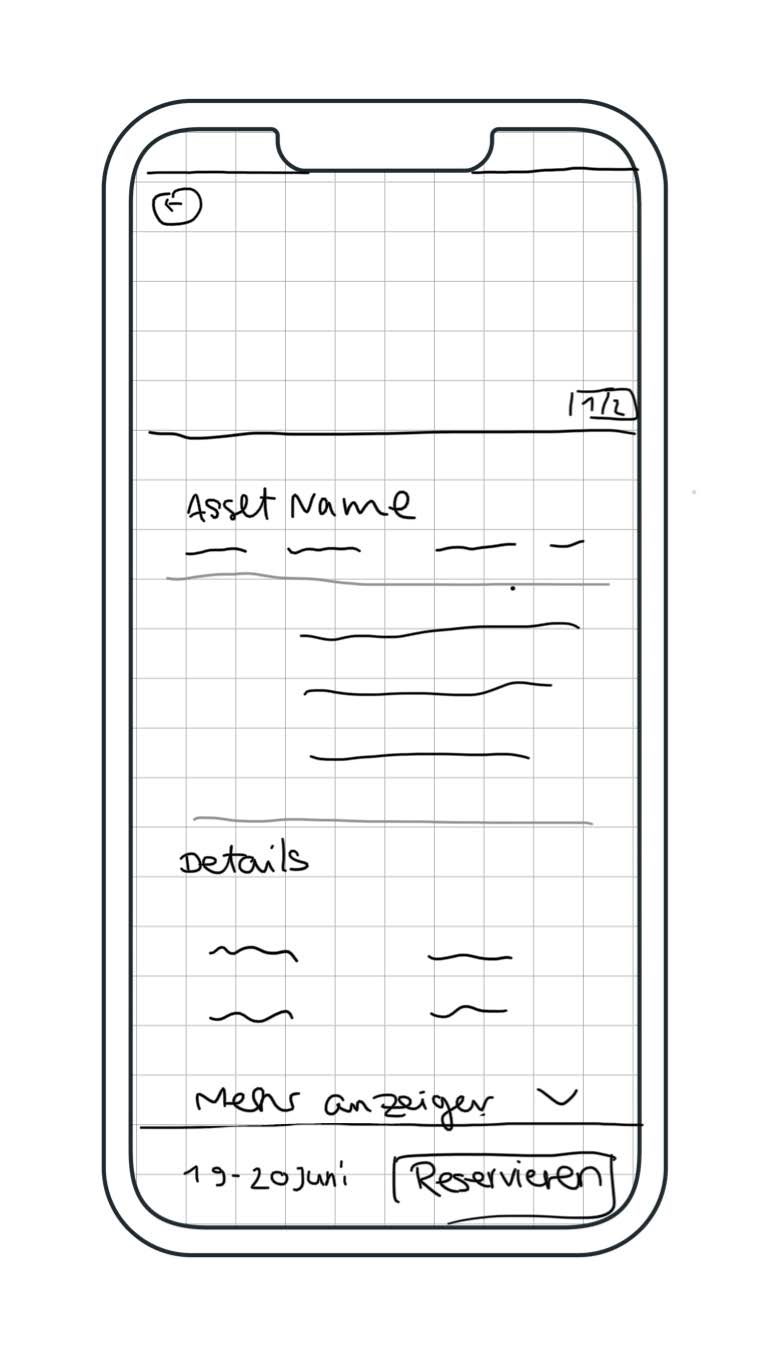
\includegraphics[scale=0.37]{Bilder/Mockups/Details.jpg}
    \label{fig:m1}
    \caption[Mockup: Kategorien, Assets, Assetdetails]{Kategorien (l), Assets (m), Assetdetails (r)}
\end{figure}


\ref{fig:m0} zeigt das Reservierungs-Checkout (Ft-A-2). Rechts ist der Kalender der Anwendung
zu sehen (Ft-A-4). 

\begin{figure}[h]
    \centering
    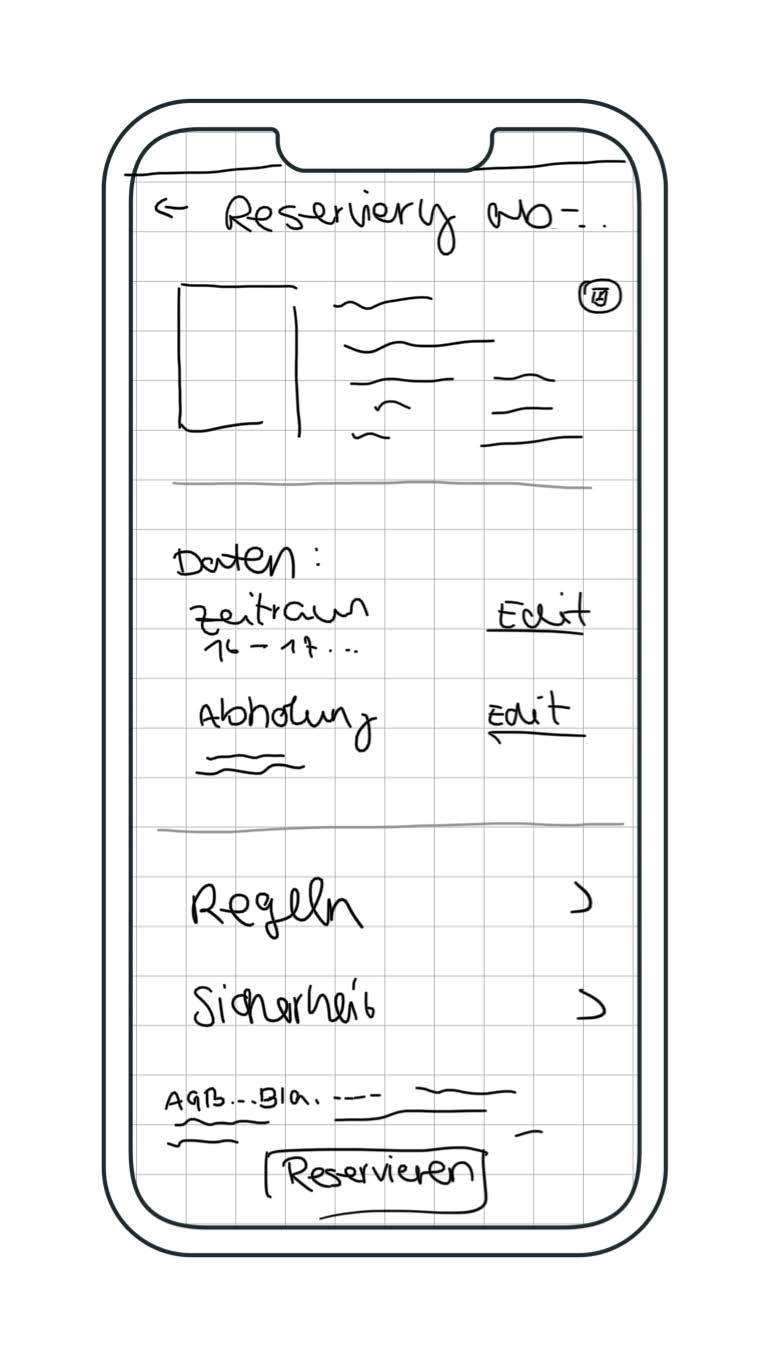
\includegraphics[scale=0.3]{Bilder/Mockups/Reservierung abschlie0en.jpg}
    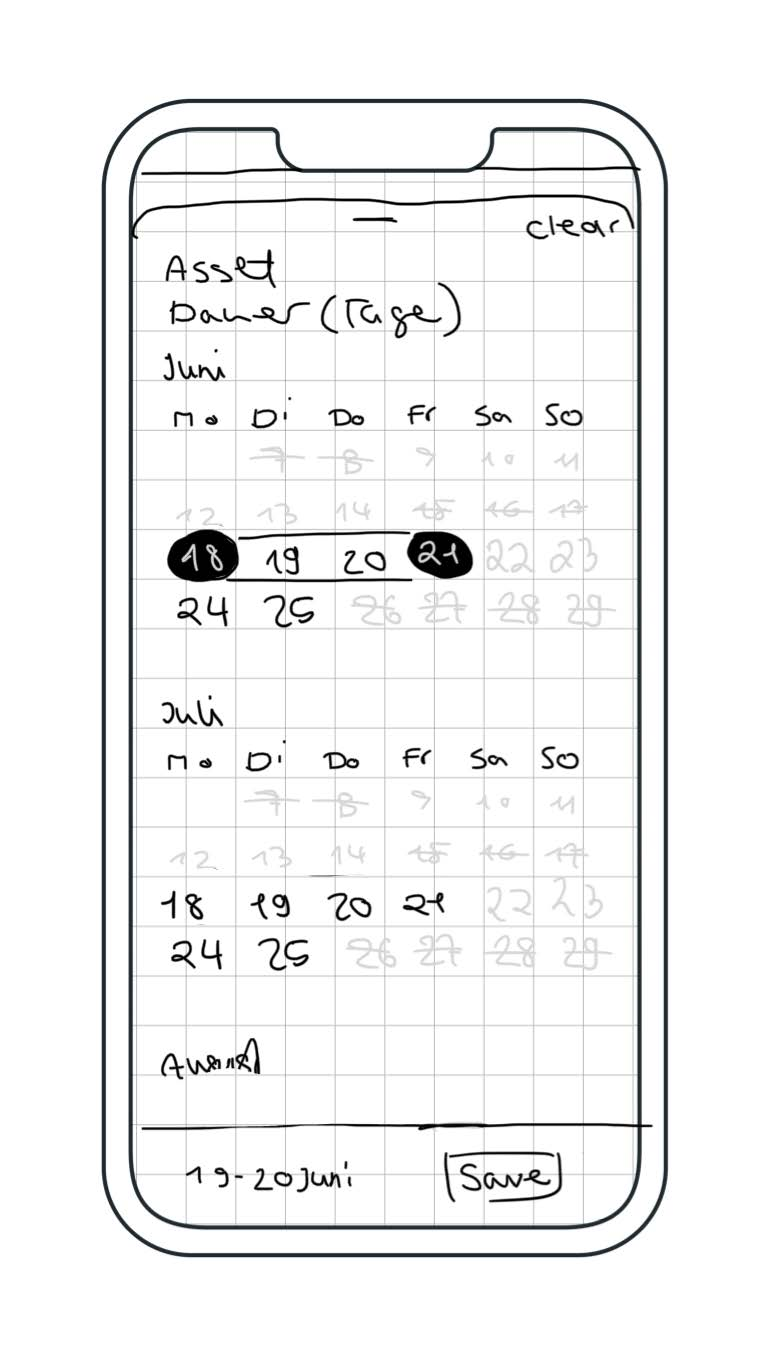
\includegraphics[scale=0.3]{Bilder/Mockups/Kalender.jpg}
    \label{fig:m3}
    \caption[Mockup: Check out, Kalender]{Check out (l), Kalender (r)}
\end{figure}

\section{Weitere Iterationen: High-Fidelity-Interface-Design}
Während des Interface-Designs wurde aus den Skizzen ein High-Fidelity-Prototyp mit
Figma\footnote{\url{https://www.figma.com/de/}} entwickelt. Der Prototyp wurden in Form einer
Usability Evaluation direkt getestet (\ref{table:e}). 



\subsection{Zwischenergebnisse}
Für die Tests wurden Usability Spezifikationen aus Szenarien abgeleitet. Die Szenarien beschreiben
Aufgaben die als Vorlage dienen. Um repetitive Evaluationsergebnisse zu verhindern, wurden die
Evaluationsergebnisse kontinuierlich in die weitere Entwicklung eingearbeitet.

\begin{table}[h]
    \centering
    \caption{Teilnehmende der Evaluation}
    \begin{tabular}{lll}
            \arrayrulecolor{maincolor}\hline
            \sffamily\color{maincolor}ID & \sffamily\color{maincolor}Alter &
            \sffamily\color{maincolor}Rolle \\
            \arrayrulecolor{maincolor}\hline
            E1                           & 19 - 25 J.                      &
            Medieninformatikerin                     \\
            E2                           & 19 - 25 J.                      & Roboterinnen \\
            E3                           & 19 - 25 J.                      & Medieninformatiker, Hilfswissenschaftler        \\
            E4                          & 19 - 25 J.                      & Medieninformatiker \\
            E5                           & 19 - 25 J.                      &
            Medieninformatikerinnen, Hilfswissenschaftlerin \\
            E6                           & 25 - 30 J.                      & Wissenschaftlicher Mitarbeiter        \\
            \arrayrulecolor{maincolor}\hline
    \end{tabular}
    \label{table:e}
\end{table}

Ein zentrales Problem des Prototyps war einen Konsistenten Wortlaut zu finden. Insbesondere der
Begriff \textit{Assets} hat zu Verwirrungen geführt, da nicht klar war, was der Begriff definiert
(E1, E2). Daraufhin wurden Vorschläge geliefert, wie \textit{Material, Hardware, Systeme, Geräte}. Im
weiteren Verlauf hat sich \textit{Material} als am verständlichsten herausgestellt (E3, E4). Des
Weiteren hat das \textit{Suchen nach Kriterien} für Missverständnisse aufgrund des Wortlautes und
der Parallelen \textit{Suche} ergeben (E1, E2). Daher wurden auch hier verschiedene Begriffe wie
\textit{Auswahlhilfe, Suchhilfe, Kriteriensuche, Kiterienhilfe, Auwahl nach Kriterien, Ausleihhilfe}
erarbeitet. Da die Funktion im Rahmen dieser Arbeit keine Realisierung gefunden hat, wurde dies nicht
weiter ausgeführt. Aus den Problemen konnten festgestellt werden, dass im Wortlaut eine
Eindeutigkeit fehlte, welche auf für die drei Regel 2,4,5 von großer Bedeutung ist, um Fehler direkt
vorbeugen zu können und Parallelen ermöglichen zu können.

Positiv wurde stets erwähnt, dass die Anwendung sauber und nicht überladen wirkt (R8) (E1-6).


Warum Ausleihzeitraum separat zu Abholung und Rückgabe -> Impliziert das bereits

--> Anhang der Ausleihhilfe,...
\subsection{Designsprache}
Mit den gesammelten Ergebnissen wurde eine konsistente Designsprache für die Anwendung festgehalten.

\subsubsection{???}

Für die spätere Realisierung wurde sich für die Typografie direkt an Tailwind
UI\footnote{\url{https://tailwindui.com/components}} orientiert.

\subsubsection{Farbschema}

Die Farben der Anwendung (\ref{fig:farben}) werden nach dem 60-30-10 Prinzip angeordnet \cite{experience_using}. Wobei Grau
die Hauptfarbe darstellt, Weiß die Sekundär Farbe und Organe die Akzentfarbe. Als Akzentfarbe wurde
sich für Orange entschieden, da die Anwendung eine Software am \ac{imis} ist und die IMIS Farben
Orange und Blau umfassen. Nach Protypischen vergliechen und umfragen wurde sich dann für das Orange
entschieden.
\begin{figure}[h]
    \centering
    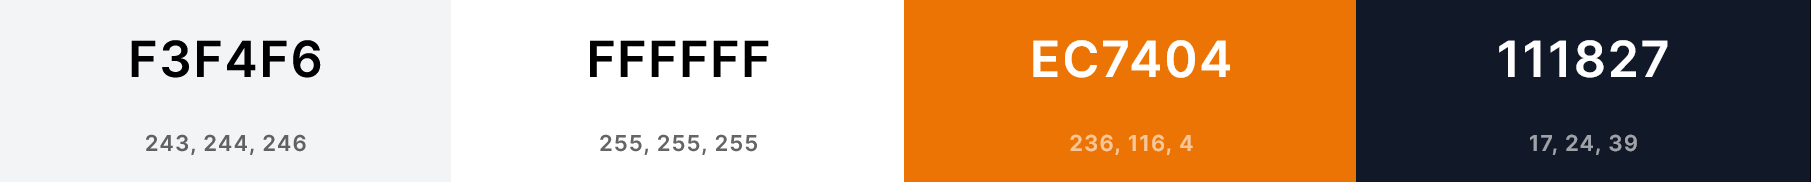
\includegraphics[scale=0.23]{Bilder/farben.png}
    \caption[Farbpalette]{Farbpalette}
    \label{fig:farben}
\end{figure}

\subsection{MIR FEHLT HIER EIN GUTER TITEL}

\subsubsection{Navigation und Suche}
In der Interface-Gestaltung gibt es verschiedene Möglichkeiten Navigation bereitzustellen. Für die
Anwendung wurde für den Mobilen Kontext eine Navigationsleiste am unteren Bildschirmrand und ein
Burgermenü oben Links oder Rechts in Erwägung gezogen. Für die Desktop-Navigation wurde zwischen
einer festen Navigationsleiste links und einer Leiste oben entscheiden. An Ende wurde sich für eine
Navigationsleiste auf der linken Seite entscheiden. Orientiert wurde sich hierbei an bekannten
Anwendungen mit ähnlichen Funktionen und dem Material Design \cite{google_material_2022}. Die
Umgangsweise mit diesen Gestaltungslösungen ist bereits bekannt und somit übertragbar (\textit{4
Beständigkeit und Standards} und \textit{6 Wiedererkennung statt Erinnerung} nach
\citeA{nielsen_enhancing_1994}).

Suche wie Google Drive, um Platz sinnvoll zu nutzen

\begin{figure}[h]
    \centering
    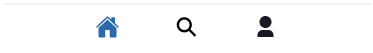
\includegraphics[scale=0.3]{Bilder/Prototyp/Property 1=Variant2.png}
    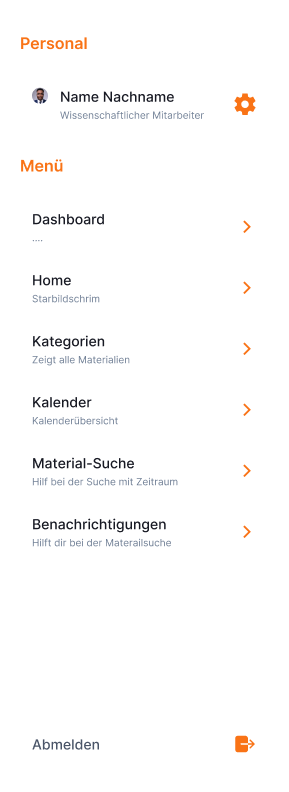
\includegraphics[scale=0.4]{Bilder/Prototyp/Menu.png}
    \caption[Farbpalette]{Navigationsmüglichkeiten}
    \label{fig:nav}
\end{figure}


\begin{figure}[h]
    \centering
    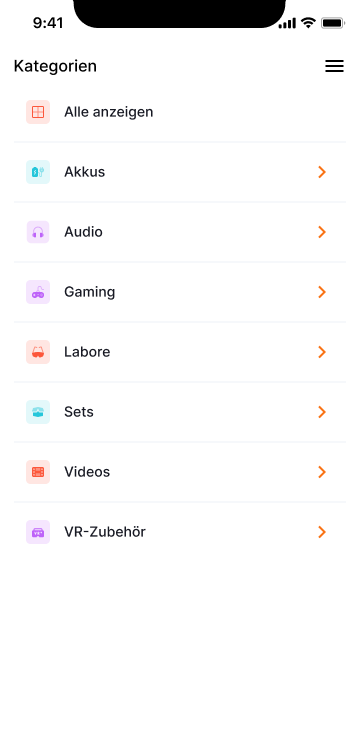
\includegraphics[scale=0.3]{Bilder/Prototyp/Kategorein 1.png}
    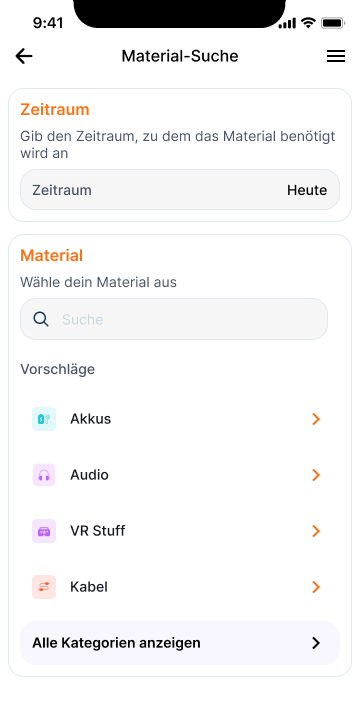
\includegraphics[scale=0.3]{Bilder/Prototyp/Suche.png}
    \label{fig:p1}
    \caption[Mockup: Kategorien, Assets, Assetdetails]{Kategorien (l), Assets (m), Assetdetails (r)}
\end{figure}


\subsubsection{Kalender}
Bei der Kalenderkomponente wurde sich direkt an dem Framework
V-Calendar\footnote{\url{https://vcalendar.io/layouts.html}} orientiert.


\begin{figure}[h]
    \centering
    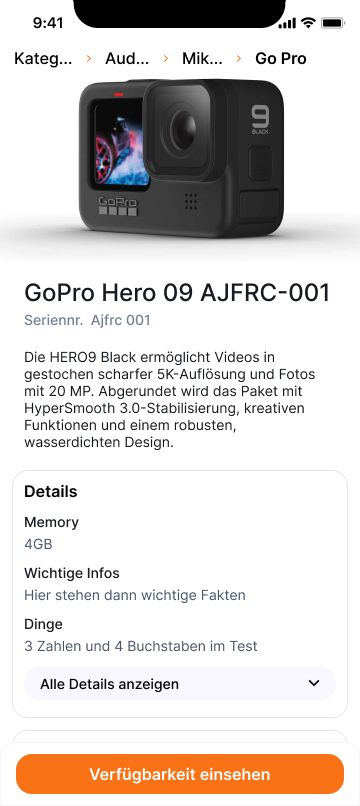
\includegraphics[scale=0.3]{Bilder/Prototyp/Datailansicht.png}
    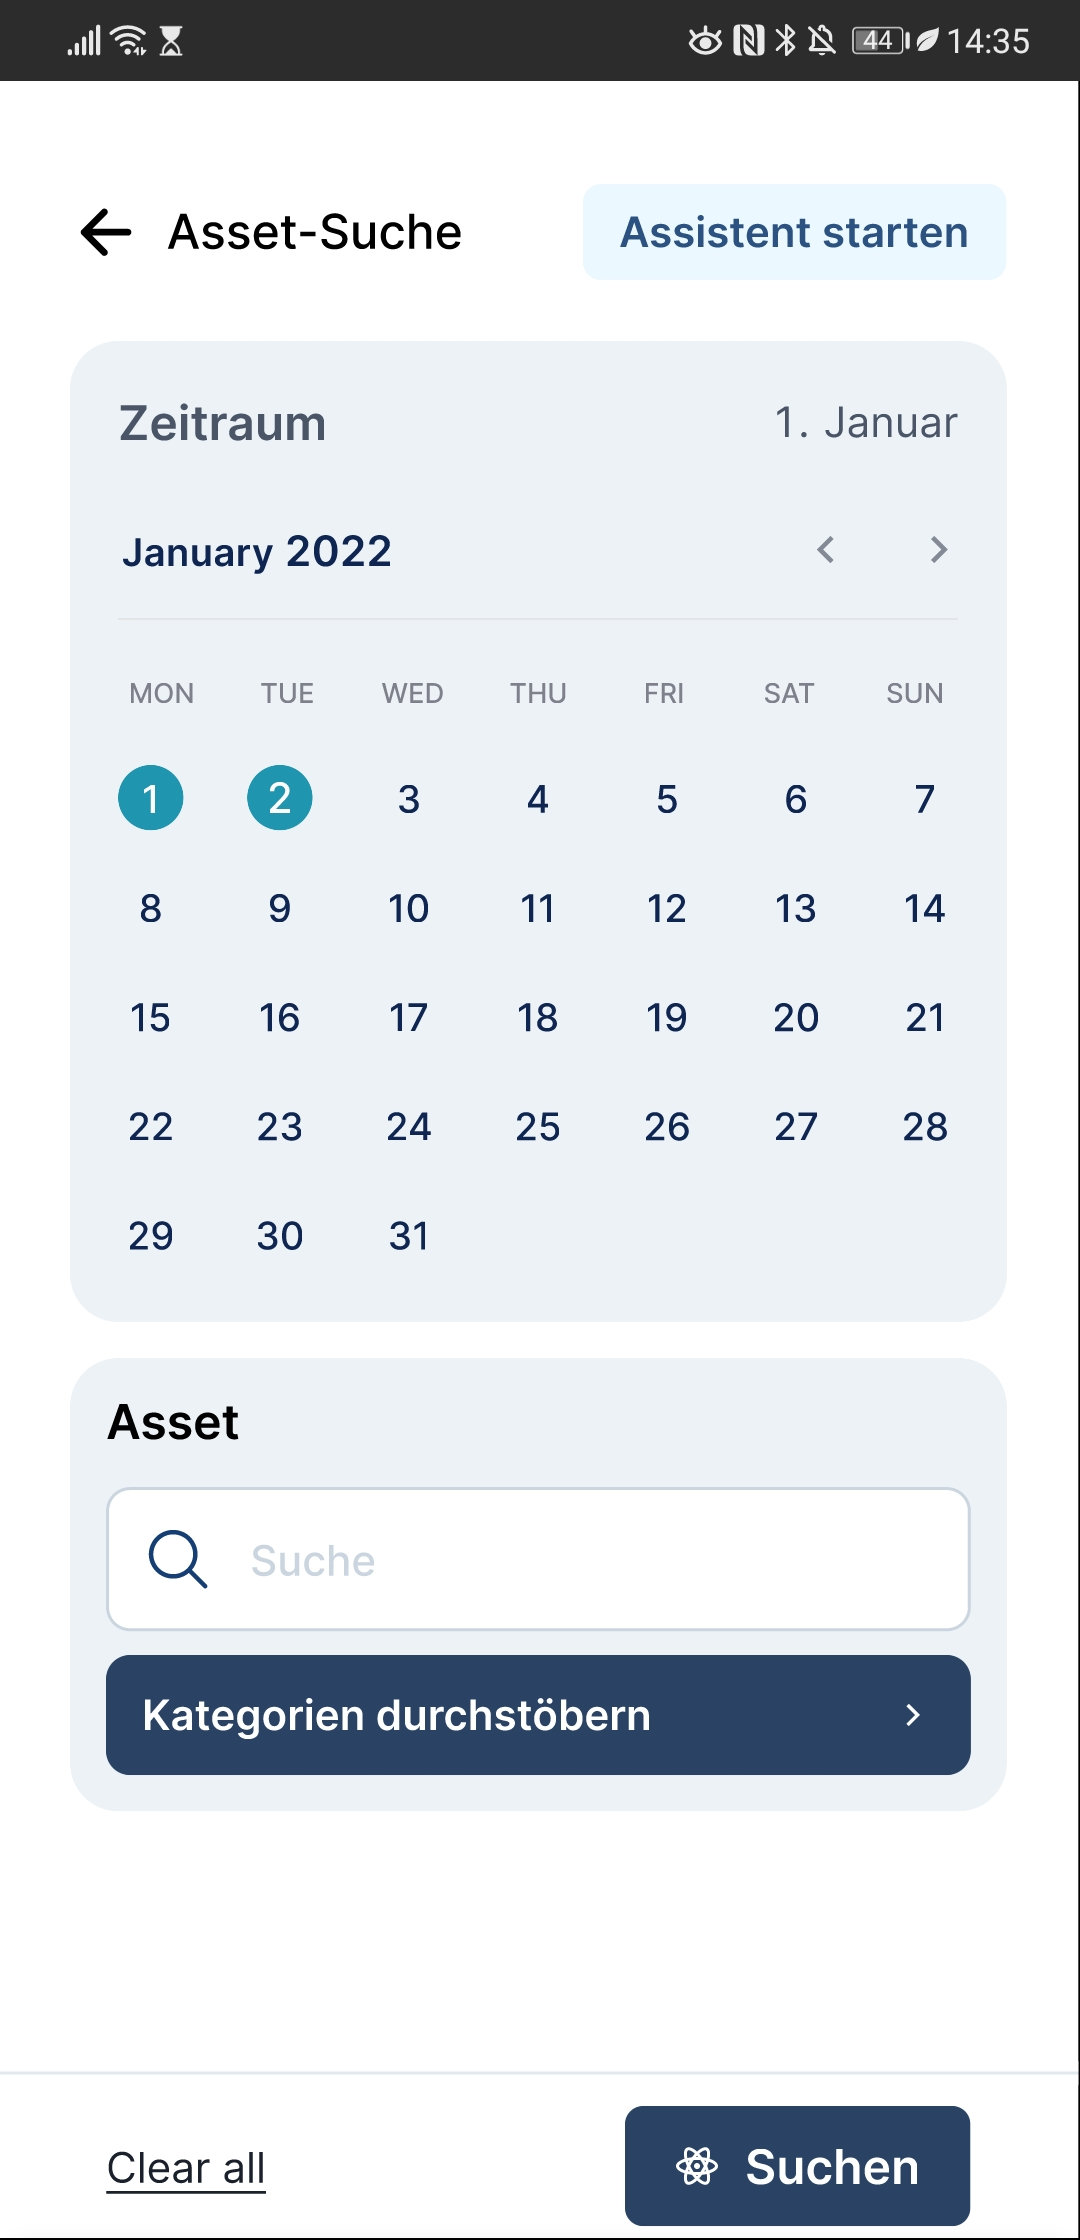
\includegraphics[scale=0.1]{Bilder/Prototyp/Kalender.jpg}
    \includegraphics[scale=0.3]{Bilder/Prototyp/Reservierung abschließen 3.png}
    \label{fig:p3}
    \caption[Mockup: Kategorien, Assets, Assetdetails]{Kategorien (l), Assets (m), Assetdetails (r)}
\end{figure}


\begin{figure}[h]
    \centering
    \includegraphics[scale=0.3]{Bilder/Prototyp/Übersicht.png}
    \includegraphics[scale=0.3]{Bilder/Prototyp/Übersicht1.png}
    \label{fig:p4}
    \caption[Mockup: Kategorien, Assets, Assetdetails]{Kategorien (l), Assets (m), Assetdetails (r)}
\end{figure}

